\section{MARCO TEORICO} 
		
\begin{enumerate}[1.]
	\item Business Analytics :
\\
\\
Al igual que la inteligencia de negocios, BA recopila y analiza datos, emplea análisis predictivos y genera informes visualizados en paneles personalizados. El objetivo de estas características es ayudar a identificar y abordar los puntos débiles de una organización. Aquí es donde terminan las similitudes. El software de análisis de negocios se utiliza para explorar y analizar datos históricos y actuales. Utiliza el análisis estadístico, la extracción de datos y el análisis cuantitativo para identificar las tendencias comerciales anteriores.
\\
Una vez que se han recopilado y analizado los datos, los sistemas de análisis de inteligencia empresarial los utilizan para el modelado predictivo. Esto puede predecir y, en la mayoría de los casos, prepararse para futuros climas empresariales. Uno de los aspectos más poderosos de BA es el informe ad-hoc, que permite a las empresas realizar análisis de datos específicos en tiempo real para responder preguntas específicas para tomar decisiones comerciales más rápidas. En efecto, el análisis de negocios utiliza el análisis predictivo para resolver problemas antes de que hayan ocurrido.

\end{enumerate}

\begin{center}
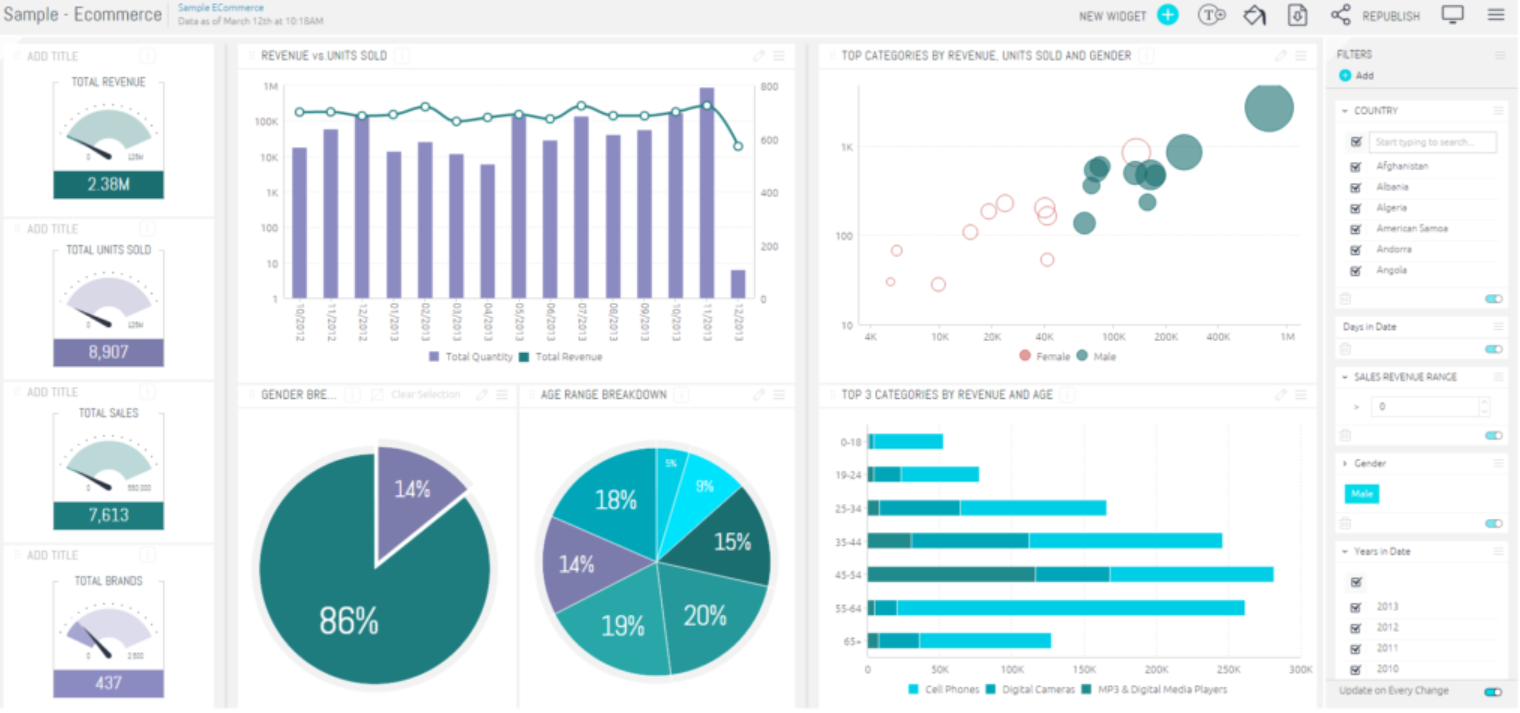
\includegraphics[scale=0.55]{./Imagenes/BA.png}
\end{center}

